% Chapter 2

\chapter{When Can One Ignore the Correlation?}
\label{ch:naive}
\lhead{Chapter~\ref{ch:naive}. \emph{When can One Ignore the Correlation?}}

\section{Problem Statement}

In the previous chapter we offer a distributed localization method dealing with unknown correlation due to lossy underwater communication. However, a \textit{na\"ive} assumption which simply ignores the correlation when fusing data from different sources, was adopted in \cite{William2015Journal,Tao2010}. It is simple in complex cooperation applications and seems to be working fine in existing works. We want to understand when this assumption is reasonable, and when is detrimental. 

There are two types of cooperative localization problems: the multi-sensor tracking problem and the multi-vehicle localization problem. The multi-sensor tracking problem is concerned with a team of cooperative nodes tracking a common target, whereas the multi-vehicle localization problem deals with a team of cooperative vehicles estimating their own positions. In both problems, individual nodes or vehicles have no idea about the whole team; they also do not share every detailed local observation. Information is shared across the team and estimation is improved over the ones with single sensor tracking or single vehicle localization (without cooperation). We illustrate the idea by exploring the information flow in the decentralized system. We quantify the situation where the correlation can be safely ignored. We would like to ensure the estimation consistency when bathymetry information is incorporated into cooperative localization.

The work in this chapter was published in~\cite{Gao2017}.

\section{Multi-Sensor Tracking Problem}

We present a simple example where two sensor nodes are tracking a common target. The central filter (CF) and single filter (SF) are used as the performance benchmarks. We answer the following questions:
\begin{itemize}
  \item What is the optimal distributed filtering?
  \item Is there any gap between the optimal distributed filtering and the central filtering? If so, what is the gap?
  \item When can one ignore the correlation in fusion? When does the \textit{na\"ive} assumption in filtering fail?
\end{itemize}

These answers give us a clear understanding about the pros and cons of implementing \textit{na\"ive} filtering (NF) in the distributed localization.

\begin{figure}[htbp]
\centering
\includegraphics[width=0.7\textwidth]{mst.png}
\caption{Multi-sensor tracking: a recursive two-step flow chart. The target propagates from previous position ${\bf x}_k$ to current position ${\bf x}_{k+1}$ with some propagation noise ${\bf \omega}_k$. At each step, each node makes an observation (${\bf z}^{(1)}$ or ${\bf z}^{(2)}$) about the target position.}
\label{fig:mst}
\end{figure}

Figure~\ref{fig:mst} shows a recursive two-step process where two sensor nodes (node 1 and 2) track a target with position state $\bf x$ of size $n\times 1$. The target propagates from previous position ${\bf x}_k$ to current position ${\bf x}_{k+1}$ with some propagation noise ${\bf \omega}_k$. At each step, each node makes an observation (${\bf z}^{(1)}$ or ${\bf z}^{(2)}$) about the target position. The propagation model and observation models are
\begin{equation}
\begin{split}
{\bf x}_{k+1}&={\bf x}_k+{\bf \omega}_k\\
{\bf z}^{(1)}_k&={\bf x}_k+{\bf \nu}^{(1)}_k \\
{\bf z}^{(2)}_k&={\bf x}_k+{\bf \nu}^{(2)}_k\\
\end{split}
\end{equation}
where the propagation noise $\bf \omega$ and observation noises ${\bf \nu}^{(1)}$ and ${\bf \nu}^{(2)}$ at all steps are independent zero-mean Gaussian processes with covariances ${\bf Q}$, ${\bf R}^{(1)}$ and ${\bf R}^{(2)}$. Without loss of generality, we assume $\det{\bf R}^{(1)}\leq\det{\bf R}^{(2)}$. The problem is to find the best estimate ${\bf y}_{k+1}$ about the target position ${\bf x}_{k+1}$. We assess the filters' one-step and asymptotic performances. With the knowledge about target position at the previous step ${\bf x}_{k}$, one-step performance is the filter performance at the next step. When filters continue to be implemented over many steps, the estimation reaches a stable state where asymptotic performance can be derived.

Assuming a central unit with access to the local sensor data in real time, the central filtering (CF) simply stacks the local observations made at two nodes and follows the Kalman filtering to update the predicted estimate about the target. Similarly, single filtering (SF) follows Kalman filtering and uses the sensor data at node 1 only without cooperation from the other node.

Let the error covariance of the position estimate about state ${\bf x}_k$ be ${\bf P}_k$. The estimate about the state ${\bf x}_k$ is ${\bf y}_k=\mathbb{E}[{\bf x}_k]$. The one-step SF gives estimate with error covariance
\begin{equation}
{\bf P}_{\text{SF}}=\big({\bf I}-({\bf P}_k+{\bf Q})({\bf P}_k+{\bf Q}+{\bf R}^{(1)})^{-1}\big)({\bf P}_k+{\bf Q})%\frac{({\bf P}_k+{\bf Q}){\bf R}^{(1)}}{{\bf P}_k+{\bf Q}+{\bf R}^{(1)}}
\end{equation}
and one-step CF gives
\begin{equation}
{\bf P}_{\text{CF}}=\big({\bf I}-({\bf P}_k+{\bf Q}){\bf H}_\text{CF}{\bf S}_\text{CF}^{-1}\big)({\bf P}_k+{\bf Q})%\frac{({\bf P}_k+{\bf Q}){\bf R}^{(1)}{\bf R}^{(2)}}{{\bf P}_k({\bf R}^{(1)}+{\bf R}^{(2)})+{\bf Q}({\bf R}^{(1)}+{\bf R}^{(2)})+{\bf R}^{(1)}{\bf R}^{(2)}}
\end{equation}
where
\begin{equation}
\begin{split}
{\bf S}_\text{CF}&={\bf H}({\bf P}_k+{\bf Q}){\bf H}_\text{CF}^\top+\left[
                                                    \begin{array}{cc}
                                                      {\bf R}^{(1)} & {\bf 0} \\
                                                      {\bf 0} & {\bf R}^{(2)} \\
                                                    \end{array}
                                                  \right]
\\
{\bf H}_\text{CF}&=\left[
           \begin{array}{c}
             {\bf I} \\
             {\bf I} \\
           \end{array}
         \right] \\
\end{split}
\end{equation}
and ${\bf I}$ is the identity matrix of size $n\times n$.
%We can see that CF is the same as fusing the observation data first, and uses the fused observation to update the predict about the target.

When the target keeps moving and observations are made at every step at the two nodes with the same settings, the filters reach stable states in which the estimation and performance approach constant values. The stable state estimation error covariances for both filters are derived by setting ${\bf P}_\text{SF}={\bf P}_k$ and ${\bf P}_\text{CF}={\bf P}_k$. In 1-dimensional space where $n=1$, they are
\begin{equation}
\begin{split}
{\bf P}_{\text{SF,ss}}&=\frac{-{\bf Q}+\sqrt{{\bf Q}^2+4{\bf Q}{\bf R}^{(1)}}}{2} \\
{\bf P}_{\text{CF,ss}}&=\frac{-{\bf Q}+\sqrt{\frac{{\bf Q}^2({\bf R}^{(1)}+{\bf R}^{(2)})+4{\bf Q}{\bf R}^{(1)}{\bf R}^{(2)}}{{\bf R}^{(1)}+{\bf R}^{(2)}}}}{2}.
\end{split}
\end{equation}
The CF result is similar to SF but at each time the observation data is fused by the two sensor data. This `fused' observation therefore has error covariance $({{\bf R}^{(1)}}^{-1}+{{\bf R}^{(2)}}^{-1})^{-1}$. \\
\indent It should be noted that the estimates by CF and SF are consistent in that the actual error covariance of the estimate $\mathbb{E}[({\bf y}-{\bf x})({\bf y}-{\bf x})^\top]$ equals the estimated error covariance $\bf P$. Therefore we only state one of them here. The performances of CF and SF are shown in the subsequent sections.

\subsection{Optimal Distributed Filtering}
\label{sec:DF}

\subsubsection{Deriving the Optimal DF}
\begin{figure}[htbp]
\centering
\includegraphics[width=0.7\textwidth]{DF.png}
\caption{Multi-sensor tracking: distributed filtering using weighted-sum fusion.}
\label{fig:DF}
\end{figure}
The recursive two-step distributed filtering is shown in Figure~\ref{fig:DF}. At the previous step $k$, sensor nodes exchange their local estimates and obtain a fused estimate ${\bf y}^{(f)}_k={\bf y}_k$ with error covariance ${\bf P}^{(f)}_k={\bf P}_k$. This fused estimate about the previous position ${\bf x}_k$ is adopted by both nodes. After that, the target position is predicted at each node locally, and updated with local sensor data  following the standard Kalman filtering method. At the current step $k+1$, again sensor nodes exchange their local estimates ${\bf y}^{(1)}_{k+1}$ and ${\bf y}^{(2)}_{k+1}$ and obtain the fused estimate ${\bf y}^{(f)}_{k+1}$. We use weighted sum to fuse the two estimates with weight $\lambda$
\begin{equation}
\begin{split}
{\bf y}^{(f)}_{\text{DF}}&=f({\bf y}^{(1)}_{k+1},{\bf y}^{(2)}_{k+1})\\
&=(1-\lambda){\bf y}^{(1)}_{k+1}+\lambda{\bf y}^{(2)}_{k+1}.
\end{split}
\end{equation}
With the fused estimate ${\bf y}^{(f)}_k$ and estimated error covariance ${\bf P}_k^{(f)}$, the local estimates are for nodes $i=1,2$
\begin{equation}
\label{eq:localupdate}
\begin{split}
{\bf y}^{(i)}&={\bf P}^{(i)}({{\bf P}_k^{(f)}}^{-1}{\bf y}_k^{(f)}+{{\bf R}^{(i)}}^{-1}{\bf z}^{(i)}_{k+1}) \\%\frac{{\bf R}_i}{{\bf R}_i+{\bf P}_k}\bar{\bf y}+\frac{{\bf P}_k}{{\bf R}_i+{\bf P}_k}{\bf z}_i\\
{\bf P}^{(i)}&=({{\bf R}^{(i)}}^{-1}+{{\bf P}_k^{(f)}}^{-1})^{-1}%\frac{{\bf R}_i{\bf P}_k}{{\bf R}_i+{\bf P}_k}
\end{split}
\end{equation}
The optimal weights $\lambda^*$ is derived by minimizing the error covariance $\mathbb{E}[({{\bf y}^{(f)}_{\text{DF}}}-{\bf x}_{k+1})({{\bf y}^{(f)}_{\text{DF}}}-{\bf x}_{k+1})^\top]$ and in 1-dimensional space we obtain
\begin{equation}
\begin{split}
\lambda^*&=\arg\min\mathbb{E}[({{\bf y}^{(f)}_{\text{DF}}}-{\bf x}_{k+1})^2]\\
&=\frac{{\bf R}^{(1)}}{{\bf R}^{(1)}+{\bf R}^{(2)}}. \\
\end{split}
\end{equation}
With this optimal weight, the error covariance $\mathbb{E}[({{\bf y}^{(f)}_{\text{DF}}}-{\bf x}_{k+1})({{\bf y}^{(f)}_{\text{DF}}}-{\bf x}_{k+1})^\top]$ of the fused estimate turns out to be identical with Bar Shalom's state vector fusion (SVF) \cite{Bar-Shalom1986}
\begin{equation}
\begin{split}
{\bf P}^{(f)}_{\text{SVF}}&={\bf P}^{(1)}_{k+1}\!-\!({\bf P}^{(1)}_{k+1}\!-\!{\bf P}^{(12)}_{k+1})({\bf P}^{(1)}_{k+1}\!+\!{\bf P}^{(2)}_{k+1}\!-\!{\bf P}^{(12)}_{k+1}\!-\!{{\bf P}^{(12)}_{k+1}}^\top)^{-1}({\bf P}^{(1)}_{k+1}\!-\!{{\bf P}^{(12)}_{k+1}}^\top)\\
\end{split}
\end{equation}
where the cross-correlation ${\bf P}^{(12)}_{k+1}\!=\!\mathbb{E}[({{\bf y}^{(1)}_{k+1}}\!-\!{\bf x}_{k+1})({{\bf y}^{(2)}_{k+1}}\!-\!{\bf x}_{k+1})^\top]$ between the two estimates is required. Although ${\bf P}^{(12)}_{k+1}$ is not required for optimal fusion of the estimate in DF, it is required for a consistent estimation on the error covariance ${{\bf P}^{(f)}_{\text{DF}}}^*$ which can be used for the subsequent steps. The stable state error covariance of optimal DF can also be derived by setting ${{\bf P}^{(f)}_{\text{DF}}}^*={\bf P}_k$.

\subsubsection{The Gap between the Optimal DF and CF}

\begin{figure}[htbp]
\centering
\includegraphics[width=.7\textwidth]{cmp_eg1.png}
\caption{One-step error covariances of DF, SF, CF and SVF, against the weight $\lambda$ used by DF. There is a gap between CF and optimal DF (SVF).}
\label{cmp_eg1}
\end{figure}

Figure~\ref{cmp_eg1} shows an example of the one-step performance comparing the error covariances of the estimates by DF, SF, CF and SVF, against the weight $\lambda$ used by DF. The optimal weight $\lambda^*$ is obtained at the lowest point of the DF curve, which gives identical performance as SVF. There is a gap between the optimal DF (or SVF) and CF. The same idea was stated by Bar-Shalom in \cite{ShalomComments}
\begin{displayquote}
\textit{The sufficient statistics for the global data set $D^{ij}=D^i\bigcup D^j$ cannot be expressed in terms of the sufficient statistics of the local data sets $D^i$ and $D^j$ (the local estimates $\hat{x}^i$ and $\hat{x}^j$)}.
\end{displayquote}
We have discussed the similarity information loss in distributed localization in Chapter~\ref{ch:distributed}. There is information loss when processed data (estimates) are transmitted instead of raw data (observations). This is because the CF is a Maximum a Posteriori (MAP) estimation which estimates the unobserved target position state $\bf x$ with two observations ${\bf z}^{(1)}$ and ${\bf z}^{(2)}$. The prior distribution is known as $\mathcal{N}({\bf x},{\bf P}_k+{\bf Q})$. In the other hand, DF treats the two local estimates ${\bf y}^{(1)}_{k+1}$ and ${\bf y}^{(2)}_{k+1}$ as two `observations'. The fusion is a Maximum Likelihood (ML) estimation without using the prior knowledge about the state \cite{Chang1997}. This is the best that distributed estimation can achieve when only local estimates are available for fusion. Therefore it is optimal only in the ML context. We take SVF as an example, since it is identical to the optimal DF. Let the error covariance of the two estimates from the nodes be
\begin{equation}
{\bf P}_{\text{SVF}}=\left[
                       \begin{array}{cc}
                         {\bf P}^{(1)}_{k+1} & {\bf P}^{(12)}_{k+1} \\
                         {{\bf P}^{(12)}_{k+1}}^\top & {\bf P}^{(2)}_{k+1} \\
                       \end{array}
                     \right]
\end{equation}
where
\begin{equation}
\begin{split}
{\bf P}_{1}&=\mathbb{E}[({{\bf y}^{(1)}_{k+1}}-{\bf x}_{k+1})({{\bf y}^{(1)}_{k+1}}-{\bf x}_{k+1})^\top]\\
{\bf P}_{2}&=\mathbb{E}[({{\bf y}^{(2)}_{k+1}}-{\bf x}_{k+1})({{\bf y}^{(2)}_{k+1}}-{\bf x}_{k+1})^\top]\\
{\bf P}^{(12)}_{k+1}&=\mathbb{E}[({{\bf y}^{(1)}_{k+1}}-{\bf x}_{k+1})({{\bf y}^{(2)}_{k+1}}-{\bf x}_{k+1})^\top]\\
\end{split}
\end{equation}
The target position ${\bf x}_{k+1}$ is to be determined based on the two `observations' ${\bf y}^{(1)}_{k+1}$ and ${\bf y}^{(2)}_{k+1}$. The logarithm of the likelihood function $\mathcal{L}({\bf x}_{k+1};{\bf y}^{(1)}_{k+1},{\bf y}^{(2)}_{k+1})$ is
\begin{equation}
\begin{split}
&\ln\mathcal{L}({\bf x}_{k+1};{\bf y}^{(1)}_{k+1},{\bf y}^{(2)}_{k+1})\\
= &\ln 2\pi-\frac{1}{2}\ln\Big(\det({\bf P}_\text{SVF}) \\
&+(\left[                                                \begin{array}{c}
{\bf y}^{(1)}_{k+1} \\
{\bf y}^{(2)}_{k+1} \\\end{array}\right]-\left[\begin{array}{c}
 {\bf x}_{k+1} \\
 {\bf x}_{k+1} \\\end{array}\right]
)^\top{\bf P}_{\text{SVF}}^{-1}(\left[
  \begin{array}{c}
{\bf y}^{(1)}_{k+1} \\
{\bf y}^{(2)}_{k+1} \\
\end{array}\right]-\left[
           \begin{array}{c}
           {\bf x}_{k+1} \\
           {\bf x}_{k+1} \\\end{array}\right])\Big).
\end{split}
\end{equation}
It is maximized by setting $\frac{\partial\mathcal{L}({\bf x}_{k+1};{\bf y}^{(1)}_{k+1},{\bf y}^{(2)}_{k+1})}{\partial{\bf x}}=0$. The optimal estimate for position state $\bf x$ in 1-dimensional space is
\begin{equation}
\begin{split}
{\bf y}^*_\text{ML}&=\arg\max\mathcal{L}({\bf x}_{k+1};{\bf y}^{(1)}_{k+1},{\bf y}^{(2)}_{k+1})\\
&=\frac{{\bf P}^{(2)}_{k+1}{\bf y}^{(1)}_{k+1}+{\bf P}^{(1)}_{k+1}{\bf y}^{(2)}_{k+1}-{\bf P}^{(12)}_{k+1}({\bf y}^{(1)}_{k+1}+{\bf y}^{(2)}_{k+1})}{{\bf P}^{(1)}_{k+1}+{\bf P}^{(2)}_{k+1}-2{\bf P}^{(12)}_{k+1}}.
\end{split}
\end{equation}

The volume ratio of the error covariances compared with CF is
\begin{equation}
\frac{\det{\bf P}^{(f)}_{\text{SVF}}}{\det{\bf P}_\text{CF}}=\frac{\det{{{\bf P}^{(f)}_{\text{DF}}}^*}}{\det{\bf P}_\text{CF}}.
\end{equation}
Figure~\ref{ratio} shows that the ratio is always less than one for $n=1$. The axes are ${\bf R}^{(1)}$ and ${\bf R}^{(2)}$ normalized by ${\bf P}_k+{\bf Q}$ .

\begin{figure}[htbp]
\centering
\includegraphics[width=0.8\textwidth]{ratio.png}
\caption{Ratio of error covariances - optimal DF (SVF) to CF is no larger than one.}
\label{ratio}
\end{figure}

\subsection{When Can One Ignore the Correlation?}
\label{sec:nf}
The \textit{na\"ive} filter (NF) simply fuses the two estimates assuming no correlation between them. The procedure is similar to DF in Figure~\ref{fig:DF} but the weight of fusion is calculated by the estimated error covariances, that is, $\lambda_\text{NF}={{\bf P}^{(1)}_{k+1}}{{\bf P}^{(f)}}^{-1}$. The fused estimate is
\begin{equation}
\begin{split}
{\bf y}^{(f)}_{\text{NF}}&=({\bf I}-\lambda_\text{NF}){\bf y}^{(1)}_{k+1}+\lambda_\text{NF}{\bf y}^{(2)}_{k+1} \\
{\bf P}^{(f)}_{\text{NF}}&=({{\bf P}^{(1)}_{k+1}}^{-1}+{{\bf P}^{(2)}_{k+1}}^{-1})^{-1}.
\end{split}
\end{equation}
The resulting error covariance of the fused estimate is $\mathbb{E}[({\bf y}^{(f)}_{\text{NF}}-{\bf x}_{k+1})({\bf y}^{(f)}_{\text{NF}}-{\bf x}_{k+1})^\top]$.

By ignoring the correlation, the common information from the two estimates is double counted in the fusion, which leads to estimation overconfidence. The estimated error covariance ${\bf P}^{(f)}_{\text{NF}}$ is smaller than the actual error covariance, that is $\det({\bf P}^{(f)}_{\text{NF}})<\det\mathbb{E}[({\bf y}^{(f)}_{\text{NF}}-{\bf x}_{k+1})({\bf y}^{(f)}_{\text{NF}}-{\bf x}_{k+1})^\top]$. In fact, the estimated error covariance is even smaller than the estimated covariance by CF. The overconfidence prevents utilization of subsequent useful information and therefore the actual error covariance of NF estimate is sometimes even worse than that of SF. In such a case, cooperation using NF is no longer advantageous. We call it the `\textit{dangerous}' region. \textit{Na\"ive} assumption fails here, that is when
\begin{equation}
\label{eq:nffail}
\det\mathbb{E}[({\bf y}^{(f)}_{\text{NF}}-{\bf x}_{k+1})({\bf y}^{(f)}_{\text{NF}}-{\bf x}_{k+1})^\top]>\det{\bf P}_{\text{SF}}.
\end{equation}
When the above inequality is not met, we consider that it is safe to use NF and one can ignore the correlation.

\subsubsection{One-step Performance}

We calculate the one-step \textit{dangerous} region when the inequality in Equation~\eqref{eq:nffail} is met. For $n=1$ the \textit{dangerous} region is derived as
\begin{equation}
\label{eq:danger}
\begin{split}
{\bar{\bf R}}^{(2)}>1\\
\frac{{\bar{\bf R}}^{(1)}}{{\bar{\bf R}}^{(2)}}+{\bar{\bf R}}^{(2)}+3{\bar{\bf R}}^{(1)}{\bar{\bf R}}^{(2)}\leq {\bar{\bf R}}^{(2)}\\
\end{split}
\end{equation}
where $\bar{\bf R}^{(1)}$ and $\bar{\bf R}^{(2)}$ are the normalized error covariances and $\bar{\bf R}^{(i)}=\bar{\bf R}^{(i)}/({\bf P}_k+{\bf Q}),i=1,2$. It is plotted in Figure~\ref{dregion}. We can see that it is safe to use the one-step NF only if both local observations have very small errors compared with the sum of the estimation error and propagation error, or when the two local sensors have comparable observation errors.

\begin{figure}[htbp]
\centering
\includegraphics[width=0.6\textwidth]{Figures/dregion.pdf}
\caption{One-step performance: the \textit{dangerous} region of implementing NF (assuming ${\bf R}^{(1)}<{\bf R}^{(2)}$).}
\label{dregion}
\end{figure}

\subsubsection{Asymptotic Performance}

\begin{figure}[htbp]
\begin{center}
\subfigure[]{
\includegraphics[width=0.7\textwidth]{nf_eg1.png}
\label{subfig:nf_eg1}
}
\subfigure[]{
\includegraphics[width=0.7\textwidth]{nf_eg2.png}
\label{subfig:nf_eg2}
}
\caption{\textit{Na\"ive} filter in stable state: (a) Actual error covariance is smaller than SF. (b) Actual error covariance eventually gets worse than SF. In both cases, NF is overconfident about its estimation. The estimated error covariance by NF is even lower than the one by CF.}
\label{fig:nf_eg}
\end{center}
\end{figure}

After the first step, if we continue to ignore the correlation and fuse the estimates with weights calculated from the estimated error covariances, the actual estimation error is likely to diverge and degrade further. Figure~\ref{fig:nf_eg} shows two cases in stable state. The blue dots are the actual (by Monte Carlo simulation) error covariances of the NF estimates. The horizontal line is the calculated asymptotic error covariances for NF estimates. The blue dashed line shows the estimated error covariances given by NF. We can see that NF is overconfident about its estimates. In Case (b), even though in the first step (Step 2) NF gives improvement over SF, its estimation error becomes larger than SF from Step 4 onward.

\begin{figure}[htbp]
\centering
\includegraphics[width=0.7\textwidth]{Figures/ssregion.pdf}
\caption{Asymptotic performance: the \textit{dangerous} region of implementing NF (assuming ${\bf R}^{(1)}\leq{\bf R}^{(2)}$).}
\label{fig:ssregion}
\end{figure}

We calculate the stable state error covariances of NF estimates. Compared with stable state SF error covariances, the asymptotic \textit{dangerous} region is plotted in Figure~\ref{fig:ssregion}. It should be noted that the asymptotic performance does not depend on initial error covariance, and therefore the axes are ${\bf R}^{(1)}$ and ${\bf R}^{(2)}$ normalized by the process noise error covariance ${\bf Q}$. The two cases in Figure~\ref{fig:nf_eg} are located in the plot. We can see that if the two local sensors have small measurement errors (compared with process noise), one can ignore the correlation.

\subsection{Summary}
In this section, we examined the performances of distributed processing in underwater multi-sensor tracking problem. We showed that the optimal distributed filter is achieved only when correlation is exactly tracked. However, there is still information loss due to transmission of the processed data instead of the raw data. We also showed the consequence of ignoring the correlation - the estimation overconfidence and estimation divergence. The actual estimation is worse than it is belived to be in the filter, and could be worse than the single filter without cooperation. We derived the \textit{dangerous} regions of implementing \textit{na\"ive} filter. This can be used as a guideline for conditions under which one can ignore the correlation for underwater cooperative tracking.

\section{Multi-Vehicle Localization}

Multi-vehicle localization can be viewed as cooperative network where each node estimates its own state. Different from multi-sensor tracking problem, there are many states to be estimated (one for each node), and there is a relative measurement relating the states of the cooperating nodes. Figure~\ref{fig:BN} shows the Bayesian network of two cooperating vehicles (Vehicle $i$ and Vehicle $j$). The unobserved position state variables are ${\bf x}_k^{(i)}$ and ${\bf x}^{(j)}_k$. The observed variables are the observations ${\bf z}_k^{(i)}$ or ${\bf z}_k^{(j)}$ made at Vehicle $i$ or $j$ locally about their positions and relative distance $r_k$ between them. $k=0,1,2,\dots$ denotes the discrete time step.
\begin{figure}[htbp]
  \centering
    \includegraphics[width=.6\textwidth]{BN.png}
      \caption{Bayesian network for cooperative localization of two vehicles: shaded nodes are observations and white nodes are unobserved position state variables.}
      \label{fig:BN}
\end{figure}

The position of Vehicle $i$ (so as Vehicle $j$) propagates as
\begin{equation}
\begin{split}
{\bf x}^{(i)}_{k+1}&=f({\bf x}^{(i)}_{k})+{\bf \omega}^{(i)}_{k} \\
&={\bf x}^{(i)}_{k}+{\bf v}^{(i)}_k+{\bf \omega}^{(i)}_{k}
\end{split}
\label{eq:mvlpropagation}
\end{equation}
where ${\bf v}$ is the known speed. The observations are
\begin{equation}
\begin{split}
{\bf z}^{(i)}_{k}&=h({\bf x}^{(i)}_{k})+{\bf \nu}^{(i)}_{k}\\
&={\bf x}^{(i)}_{k}+{\bf\nu}^{(i)}_{k}\\
{\bf z}^{(j)}_{k}&=h({\bf x}^{(j)}_{k})+{\bf \nu}^{(j)}_{k}\\
&={\bf x}^{(j)}_{k}+{\bf\nu}^{(j)}_{k}\\
r_{k}&={\bf x}^{(i)}_{k}-{\bf x}^{(j)}_{k}+\upsilon_{k}\\
\end{split}
\label{eq:mvlmeasurement}
\end{equation}
%The Bayesian network is shown in Figure~\ref{fig:BN}.

\subsection{Information Flow when Ignoring Correlation}

Assuming all the noises and priors are Gaussian distributed, the joint Gaussian distribution of state $\bf x$ and observations ${\bf z}$ is given by
\begin{equation}
\text{Prob}(\left[                                             \begin{array}{c}
                                  {\bf x} \\
                                {\bf z} \\
                  \end{array}
                \right])=\alpha e^{\frac{1}{2}}(\left[
                          \begin{array}{c}
                        {\bf x} \\
                    {\bf z} \\
                  \end{array}
                \right]-{\bf\mu})^\top{\bf \Lambda}(\left[                   \begin{array}{c}
                       {\bf x} \\            
                       {\bf z} \\           \end{array}  \right]-{\bf\mu})
\end{equation}
where $\mu=\left[\begin{array}{c}               \mu_{\bf x} \\                 \mu_{\bf z} \\            \end{array}\right]=\left[\begin{array}{c}               \mathbb{E}({\bf x}) \\                 \mathbb{E}({\bf z}) \\            \end{array}\right]$ and $\bf \Lambda$ is the precision matrix (or inverse covariance matrix). ${\bf\Lambda}$ has the following blockwise structure:
\begin{equation}
{\bf \Lambda}=\left[
          \begin{array}{cc}
            {\bf \Lambda}_{\bf xx} & {\bf \Lambda}_{xz} \\
            {\bf \Lambda}_{zx} & {\bf \Lambda}_{zz} \\
          \end{array}
        \right]={\bf P}^{-1}
\end{equation}
where $\bf P$ is the covariance matrix for $\left[                                             \begin{array}{c}
                                  {\bf x} \\
                                {\bf z} \\
                  \end{array}
                \right]$ and ${\bf P}=\left[
          \begin{array}{cc}
            {\bf P}_{\bf xx} & {\bf P}_{\bf xz} \\
            {\bf P}_{\bf zx} & {\bf P}_{\bf zz} \\
          \end{array}
        \right]$. It should be noted that the subscripts of the subblocks ${\bf \Lambda}_{\bf xx}$, ${\bf \Lambda}_{\bf xz}={\bf \Lambda}_{\bf zx}^\top$ and ${\bf \Lambda}_{\bf zz}$ are denote the sizes corresponding to $\bf x$ and $\bf z$. ${\bf \Lambda}_{\bf xx}^{-1}$ is the conditional covariance of $\bf x$ given all the observations $\bf z$. It describes the covariance of the Gaussian probability $p({\bf x}|{\bf z})$. We define the conditional covariance as
        \begin{equation}
        \begin{split}
        {\bf C}_{\bf x|z}&={\bf \Lambda}_{\bf xx}^{-1}\\
        &={\bf P}_{\bf xx}-{\bf P}_{\bf xz}{\bf P}_{\bf zz}^{-1}{\bf P}_{\bf zx}.
        \end{split}
        \end{equation}
This is also the result of block matrix inversion. We also have
\begin{equation}
{\bf P}_{\bf xx}^{-1}={\bf \Lambda}_{\bf xx}-{\bf \Lambda}_{\bf xz}{\bf \Lambda}_{\bf zz}^{-1}{\bf \Lambda}_{\bf xz}^\top.
\end{equation}
When ${\bf z}$ are linear observations about $\bf x$, ${\bf z}={\bf H}{\bf x}+{\bf \nu}$, we have ${\bf z}\sim\mathcal{N}({\bf H}{\bf x}, {\bf R})$ and
\begin{equation}
\begin{split}
{\bf P}_{\bf xz}&={\bf P}_{\bf zx}^\top={\bf P}_{\bf xx}{\bf H}^\top \\
{\bf P}_{\bf zz}&={\bf H}{\bf P}_{\bf xx}{\bf H}^\top+{\bf R} \\
        {\bf \Lambda}_{\bf xx}&={\bf H}^\top{\bf R}^{-1}{\bf H}+{\bf P}_{\bf xx}^{-1}\\
        {\bf \Lambda}_{\bf xz}&=-{\bf \Lambda}_{\bf xx}{\bf P}_{\bf xz}{\bf P}_{\bf zz}^{-1}\\
        &=-({\bf H}^\top{\bf R}^{-1}{\bf H}+{\bf P}_{\bf xx}^{-1}){\bf P}_{\bf xx}{\bf H}^\top({\bf H}{\bf P}_{\bf xx}{\bf H}^\top+{\bf R})^{-1} \\
        &=-({\bf H}^\top{\bf R}^{-1}{\bf H}{\bf P}_{\bf xx}{\bf H}^\top+{\bf H}^\top)({\bf H}{\bf P}_{\bf xx}{\bf H}^\top+{\bf R})^{-1} \\
         &=-({\bf H}^\top{\bf R}^{-1}{\bf H}{\bf P}_{\bf xx}{\bf H}^\top+{\bf H}^\top{\bf R}^{-1}{\bf R})({\bf H}{\bf P}_{\bf xx}{\bf H}^\top+{\bf R})^{-1} \\
          &=-{\bf H}^\top{\bf R}^{-1}({\bf H}{\bf P}_{\bf xx}{\bf H}^\top+{\bf R})({\bf H}{\bf P}_{\bf xx}{\bf H}^\top+{\bf R})^{-1} \\
        &=-{\bf H}^\top{\bf R}^{-1}\\
        {\bf \Lambda}_{\bf zz}^{-1}&=\bf R.\\
\end{split}
\end{equation}
The probability distribution of $\bf x$ given $\bf z$ is given by Bayesian Theorem
\begin{equation}
\begin{split}
\label{eq:pxz}
p({\bf x}|{\bf z})&=\frac{p({\bf z}|{\bf x})p({\bf x})}{p({\bf z})} \\
&=(2\pi)^{-\frac{n_{\bf z}}{2}}{\bf R}^{-\frac{1}{2}}\exp\{-\frac{1}{2}({\bf z}-{\bf H}{\bf x})^\top
{\bf R}^{-1}({\bf z}-{\bf H}{\bf x})\}\\
\times&(2\pi)^{-\frac{n_{\bf x}}{2}}{\bf P}_{\bf xx}^{-\frac{1}{2}}\exp\{-\frac{1}{2}({\bf x}-\mu_{\bf x})^\top
{\bf P}_{\bf xx}^{-1}({\bf x}-\mu_{\bf x})\} \\
\times&(2\pi)^{\frac{n_{\bf z}}{2}}{\bf P}_{\bf zz}^{\frac{1}{2}}\exp\{\frac{1}{2}({\bf z}-\mu_{\bf z})^\top
{\bf P}_{zz}^{-1}({\bf z}-\mu_{\bf z})\}. \\
\end{split}
\end{equation}
We examine the exponents and look for an estimated mean ${\bf\hat x}$ about $\bf x$ given $\bf z$, such that $p(\bf x|\bf z)$ is maximized. The maximum $\ln p(\bf x|\bf z)$ is found by taking the derivative $\frac{\partial\ln p(\bf x|\bf z)}{\partial\bf x}=0$. Therefore in Equation~\eqref{eq:pxz} we are only interested in the exponent terms involving $\bf x$. We are now left with
\begin{equation}
\begin{split}
&-\frac{1}{2}({\bf z}-{\bf H}{\bf x})^\top
{\bf R}^{-1}({\bf z}-{\bf H}{\bf x})-\frac{1}{2}({\bf x}-\mu_{\bf x})^\top
{\bf P}_{\bf xx}^{-1}({\bf x}-\mu_{\bf x})\\
=&-\frac{1}{2}[{\bf z}^\top{\bf R}^{-1}{\bf z}+{\bf x}^\top{\bf H}^\top{\bf R}^{-1}{\bf H}{\bf x}-{\bf z}^\top{\bf R}^{-1}{\bf H}{\bf x}-{\bf x}^\top{\bf H}^\top{\bf R}^{-1}{\bf z} \\
&+{\bf x}^\top{\bf P}_{\bf xx}^{-1}{\bf x}-{\bf x}^\top{\bf P}_{\bf xx}^{-1}\mu_{\bf x}-\mu_{\bf x}^\top{\bf P}_{\bf xx}{\bf x}+\mu_{\bf x}^\top{\bf P}_{\bf xx}\mu_{\bf x}].
\end{split}
\end{equation}
Again we drop the terms not involving $\bf x$. We group the similar terms with respect to ${\bf x}$ and denote it as a function of $\bf x$, that is
\begin{equation}
\begin{split}
g(\bf x)&=-\frac{1}{2}[{\bf x}^\top({\bf H}^\top{\bf R}^{-1}{\bf H}+{\bf P}_{\bf xx}^{-1}){\bf x}-({\bf z}^\top{\bf R}^{-1}{\bf H}+\mu_{\bf x}^\top{\bf P}_{\bf xx}){\bf x}-{\bf x}^\top({\bf H}^\top{\bf R}^{-1}{\bf z}+{\bf P}_{\bf xx}^{-1}\mu_{\bf x})]\\
&=-\frac{1}{2}[{\bf x}^\top{\bf A}{\bf x}-{\bf b}^\top{\bf x}-{\bf x}^\top{\bf b}]
\end{split}
\end{equation}
where ${\bf A}={\bf H}^\top{\bf R}^{-1}{\bf H}+{\bf P}_{\bf xx}^{-1}={\bf \Lambda}_{\bf xx}$ is symmetrical and ${\bf b}={\bf H}^\top{\bf R}^{-1}{\bf z}+{\bf P}_{\bf xx}^{-1}\mu_{\bf x}=-{\bf \Lambda}_{xz}{\bf z}+{\bf P}_{\bf xx}^{-1}\mu_{\bf x}$. We can denote $\ln p({\bf x}|{\bf z})={\bf\mathcal{ B}}+g(\bf x)$ where ${\bf\mathcal{ B}}$ groups all the terms not involving $\bf x$. The solution of ${\bf \hat x}$ is found such that
\begin{equation}
\begin{split}
\frac{\partial\ln p(\bf x|\bf y)}{\partial\bf x}&=\frac{\partial({\bf\mathcal{B}}+f(\bf x))}{\partial\bf x} \\
&=\frac{\partial f(\bf x)}{\partial\bf x} \\
&=-\frac{1}{2}(\frac{\partial{\bf x}^\top{\bf A}{\bf x}}{\partial{\bf x}}-\frac{\partial{\bf b}^\top{\bf x}}{\partial{\bf x}}-\frac{\partial{\bf x}^\top{\bf b}}{\partial{\bf x}})\\
&=-\frac{1}{2}[{\bf x}^\top({\bf A}+{\bf A}^\top)-{\bf b}^\top-{\bf b}^\top] \\
&=-({\bf x}^\top{\bf A}-{\bf b}^\top) \\
&=0
\end{split}
\end{equation}
Therefore we have ${\bf A}{\bf\hat x}={\bf b}$. Substituting everything back, we have the exact inference about ${\bf x}$ given all observations $\bf z$ as a solution to:
\begin{equation}
\label{eq:EI}
{\bf \Lambda}_{\bf xx}{\bf\hat x}={\bf P}_{\bf xx}^{-1}\mu_{\bf x}-{\bf \Lambda}_{xz}{\bf z}.
\end{equation}
The exact estimation can be obtained through Kalman filtering step by step. We convert the Bayesian network in Figure~\ref{fig:BN} into Markov net where only unobserved state variables are shown (Figure~\ref{subfig:PMNk2}). 

A central filtering stacks the state variables and observations such that
\begin{equation}
\begin{split}
    {\bf x}=&[{{\bf x}^{(i)}_{k}}^\top, {{\bf x}^{(j)}_{k}}^\top, \ldots, {{\bf x}^{(i)}_{1}}^\top, {{\bf x}^{(j)}_{1}}^\top, {{\bf x}^{(i)}_{0}}^\top, {{\bf x}^{(j)}_{0}}^\top]^\top \\
    {\bf z}=&[{{\bf z}^{(i)}_{k}}^\top, {{\bf z}^{(j)}_{k}}^\top, {\bf r}_{k}^\top, \ldots, {{\bf z}^{(i)}_{1}}^\top, {{\bf z}^{(j)}_{1}}^\top, {\bf r}_{1}^\top, {{\bf z}^{(i)}_{0}}^\top, {{\bf z}^{(j)}_{0}}^\top, {\bf r}_{0}^\top]^\top
\end{split}
\end{equation}
with variables at the last (current) step $k$ as the first elements. We are interested to know the estimated mean about state ${\bf x}^{(i)}_{k}$. In the case of 1-dimensional space, we define the estimated error covariance corresponding to ${\bf x}^{(i)}_{k}$ as $\sigma^2$ and $\sigma^2={\bf C}_{{\bf x}|{\bf z}}(1,1)$. We define the error covariance of the estimated mean for state ${\bf x}^{(i)}_{k}$ as $\delta^2$ and $\delta^2=\mathbb{E}[({\bf\hat x}^{(i)}_k-{\bf x}^{(i)}_{k})^2]$. The central Kalman filter has all information about the state and observations. Therefore we have an optimal filter which utilizes information fully and gives exact estimation performance as the estimated error covariance, that is $\sigma^2=\delta^2$.

%\begin{figure}[H]
 % \centering
%    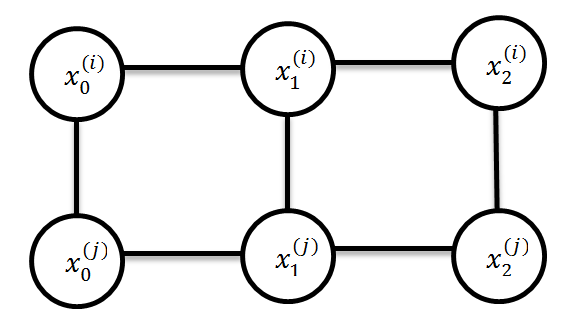
\includegraphics[width=.6\textwidth]{MN.png}
%      \caption{Markov net for cooperative localization of two vehicles. The observation nodes are omitted.}
 %     \label{fig:PMN}
%\end{figure}

%It can be seen that ${\bf \Lambda}_{\bf xz}$ are zeros everywhere but the block diagonals corresponding to each pair of sets $[{x}_{A,i}^\top, {x}_{B,i}^\top]^\top$ and $[{y}_{A,i}^\top, {y}_{B,i}^\top, {y}_{r,i}^\top]^\top$.


%\section{Unwrapped Graphical Model with Information Double Counting}
%\label{sec:unwrapped}

A distributed \textit{na\"ive} filter simply ignores the inter-vehicle correlation and treats the information from the two vehicles as independent. We represent the estimation which ignores the correlation by unwrapping the full graphic model. We show how the \textit{na\"ive} filtering deviates from the central estimator. The unwrapped network has all symbols with a tilde on top, for example, estimated mean is $\tilde\mu$, estimated covariance is $\tilde\sigma^2$, and actual error covariance is $\tilde\delta^2$ of the estimated mean.

\begin{figure}[htbp]
\begin{center}
\subfigure[Full graph (k=1).]{
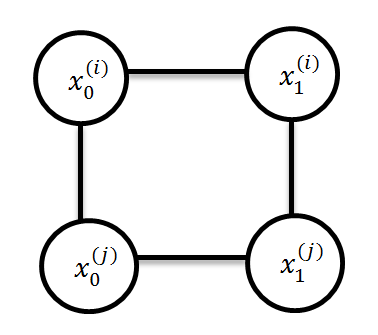
\includegraphics[width=0.45\textwidth]{MNk1}
\label{subfig:PMNk1}
}
\subfigure[Unwrapped graph (k=1).]{
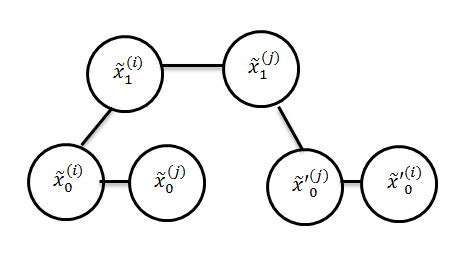
\includegraphics[width=0.45\textwidth]{UNMNk1}
\label{subfig:UNPMNk1}
}
\subfigure[Full graph (k=2).]{
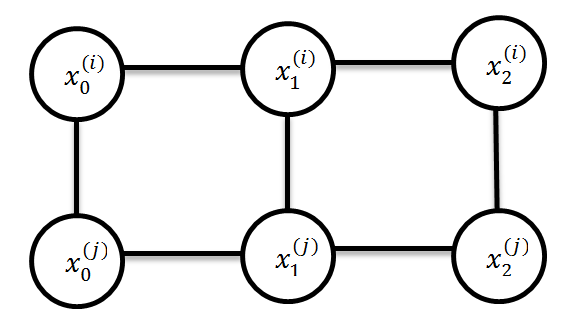
\includegraphics[width=0.65\textwidth]{MN}
\label{subfig:PMNk2}
}
\subfigure[Unwrapped graph (k=2).]{
\includegraphics[width=0.8\textwidth]{UNMNk2}
\label{subfig:UNMNk2}
}
\caption{Full graph vs. Unwrapped graph with information double counting for $k=1,2$: the prime symbol indicates the replication of nodes.}
\label{fig:LOOPYvsUN}
\end{center}
\end{figure}

We plot the unwrapped graphs in Figure~\ref{fig:LOOPYvsUN} for $k=1,2$. It can be seen that the unwrapping simply replicates the past nodes exponentially with ${\bf x}^{(i)}_{k}$ and ${\bf x}^{(j)}_{k}$ being the root nodes. The unwrapped structure assumes the duplicated nodes are from independent sources (independent priors and observations). The exact inference for the unwrapped network is obtained by
\begin{equation}
\label{eq:tildeEI}
\tilde{\bf \Lambda}_{\bf xx}{\bf{\hat{\tilde x}}}=\tilde{\bf P}_{\bf xx}^{-1}\tilde\mu_{\bf x}-\tilde{\bf \Lambda}_{\bf xz}\tilde{\bf z}.
\end{equation}
The replication from the original full network is represented by the mapping matrices ${\bf O}_{\bf x}$ and ${\bf O}_{\bf z}$ such that
\begin{equation}
\begin{split}
{\bf\tilde x}&={\bf O}_{\bf x}{\bf x} \\
{\bf\tilde z}&={\bf O}_{\bf z}{\bf z}. \\
\end{split}
\end{equation}
For example, for $k=1$, the mapping matrices are
\begin{equation}
\begin{split}
{\bf O}_{\bf x}&=\left[
             \begin{array}{cc}
               \bf 1 & \bf 0 \\
               \bf 0 & \bf 1 \\
               \bf 0 & \bf 1 \\
             \end{array}
           \right]=\left[
               \begin{array}{cccc}
                 1 & 0 & 0 & 0 \\
                 0 & 1 & 0 & 0 \\
                 0 & 0 & 1 & 0 \\
                 0 & 0 & 0 & 1 \\
                 0 & 0 & 1 & 0 \\
                 0 & 0 & 0 & 1 \\
               \end{array}
             \right]\\
{\bf O}_{\bf z}&=\left[
             \begin{array}{cc}
               \bf 1 & \bf 0 \\
               \bf 0 & \bf 1 \\
               \bf 0 & \bf 1 \\
             \end{array}
           \right]=\left[
               \begin{array}{cccccc}
                 1 & 0 & 0 & 0 & 0 & 0\\
                 0 & 1 & 0 & 0 & 0 & 0\\
                 0 & 0 & 1 & 0 & 0 & 0\\
                 0 & 0 & 0 & 1 & 0 & 0\\
                 0 & 0 & 0 & 0 & 1 & 0\\
                 0 & 0 & 0 & 0 & 0 & 1\\
                 0 & 0 & 0 & 1 & 0 & 0\\
                 0 & 0 & 0 & 0 & 1 & 0\\
                 0 & 0 & 0 & 0 & 0 & 1\\
               \end{array}
             \right]
\end{split}
\end{equation}
where the bold zeros and ones are the block zero matrix and identity matrix respectively, in appropriate sizes ($2\times 2$ for ${\bf O}_{\bf x}$ and $3\times 3$ for ${\bf O}_{\bf z}$). For $k=2$, we have
\begin{equation}
{\bf O}_{\bf x}=\left[
             \begin{array}{ccc}
               \bf 1 & \bf 0 & \bf 0 \\
               \bf 0 & \bf 1 & \bf 0 \\
               \bf 0 & \bf 0 & \bf 1 \\
                \bf 0 & \bf 1 & \bf 0 \\
               \bf 0 & \bf 0 & \bf 1 \\
               \bf 0 & \bf 0 & \bf 1 \\
               \bf 0 & \bf 0 & \bf 1 \\
             \end{array}
           \right]. \\
\end{equation}

In the mapping, state variables $\tilde{\bf x}_{i}$, $\tilde{\bf x}_{i}'$, $\tilde{\bf x}_{i}''$ and so on are copies of ${\bf x}_{i}$; so are the observations. However, the unwrapped network enables a way for the estimation not to count in the duplication. The independence assumptions are reflected in the structure of $\tilde{\bf \Lambda}$. The precision matrix ($\bf \Lambda$ or $\tilde{\bf \Lambda})$ describes the pairwise statistical relationship given all other nodes. In a Markov network, the entries of precision matrix are only nonzero for neighboring nodes. The relationship between the precision matrices $\bf\tilde \Lambda$ and $\bf \Lambda$ is listed below:
\begin{enumerate}
  \item \underline{${\tilde{\bf \Lambda}}_{\bf xz}{\bf O}_{\bf z}={\bf O}_{\bf x}{\bf \Lambda}_{\bf xz}$ and ${{\bf \Lambda}}_{\bf xz}{\bf O}_{\bf z}^\top={\bf O}_{\bf x}^\top\tilde{\bf \Lambda}_{\bf xz}$:} as ${\bf \Lambda}_{\bf xz}$ is block-diagonal and the block diagonals of $\tilde{\bf \Lambda}_{\bf xz}$ are simply replicates of the block diagonals of ${\bf \Lambda}_{\bf xz}$. ${\bf \Lambda}_{\bf xz}$ and $\tilde{\bf \Lambda}_{\bf xz}$ are equal after partially being projected to each other's domain.
  \item \underline{${\bf \Lambda}_{\bf zz}$ and $\tilde{\bf \Lambda}_{\bf zz}$ are diagonal matrices  and ${\bf O}_{\bf z}{\bf \Lambda}_{\bf zz}^{-1}=\tilde{\bf \Lambda}_{\bf zz}^{-1}{\bf O}_{\bf z}$:} ${\bf \Lambda}_{\bf zz}^{-1}$ is the diagonal observation error covariance matrix. $\tilde{\bf \Lambda}_{\bf zz}^{-1}$ replicates the block diagonals (set of observations) of ${\bf \Lambda}_{\bf zz}^{-1}$. Similarly, ${\bf \Lambda}_{\bf zz}^{-1}$ and $\tilde{\bf \Lambda}_{\bf zz}^{-1}$ are equal after partially being projected to each other's domain.
  \item \underline{An error matrix $\bf E$ is defined such that ${\tilde{\bf \Lambda}}_{\bf xx}{\bf O}_{\bf x}+{\bf E}={\bf O}_{\bf x}{\bf \Lambda}_{\bf xx}$:} the row of $\bf E$ consists all zeros for the nodes who have the same neighbors in the unwrapped network as the original nodes in the full network.
  \item \underline{${\bf E}=-(\tilde{\bf P}_{\bf xx}^{-1}{\bf O}_{\bf x}-{\bf O}_{\bf x}{\bf P}_{\bf xx}^{-1})$:} the property is proved by using block matrix inversion and the relationship summarized above.
\end{enumerate}

\begin{proof}%[Proof of ${\bf E}=-(\tilde{\bf P}_{\bf xx}^{-1}{\bf O}_{\bf x}-{\bf O}_{\bf x}{\bf P}_{\bf xx}^{-1})$]


Using the block matrix inversions
\begin{equation*}
\begin{split}
{\bf P}_{\bf xx}^{-1}&={\bf \Lambda}_{\bf xx}-{\bf \Lambda}_{\bf xz}{\bf \Lambda}_{\bf zz}^{-1}{\bf \Lambda}_{\bf xz}^\top, \\
\tilde{\bf P}_{\bf xx}^{-1}&=\tilde{\bf \Lambda}_{\bf xx}-\tilde{\bf \Lambda}_{\bf xz}\tilde{\bf \Lambda}_{\bf zz}^{-1}\tilde{\bf \Lambda}_{\bf xz}^\top,\\
\end{split}
\end{equation*}
we have
\begin{align*}
%\begin{eqnarray*}
&{\bf O}_{\bf x}({\bf \Lambda}_{\bf xx}-{\bf P}_{\bf xx}^{-1})-(\tilde{\bf \Lambda}_{\bf xx}-\tilde{\bf P}_{\bf xx}^{-1}){\bf O}_{\bf x} & \\
=&{\bf O}_{\bf x}\underline{{\bf \Lambda}_{\bf xz}{\bf \Lambda}_{\bf zz}^{-1}{\bf \Lambda}_{\bf xz}^\top}-\underline{\tilde{\bf \Lambda}_{\bf xz}\tilde{\bf \Lambda}_{\bf zz}^{-1}\tilde{\bf \Lambda}_{\bf xz}^\top}{\bf O}_{\bf x} & \textrm{by block matrix inversion}\\
=&\underline{\tilde{\bf \Lambda}_{\bf xz}{\bf O}_{\bf z}}{\bf \Lambda}_{\bf zz}^{-1}{\bf \Lambda}_{\bf xz}^\top-\tilde{\bf \Lambda}_{\bf xz}\tilde{\bf \Lambda}_{\bf zz}^{-1}\underline{{\bf O}_{\bf z}{\bf \Lambda}_{\bf xz}^\top} & \textrm{by relationship between ${\bf \Lambda}_{\bf xz}$ and $\tilde{\bf \Lambda}_{\bf xz}$}\\
=&\tilde{\bf \Lambda}_{\bf xz}({\bf O}_{\bf z}{\bf \Lambda}_{\bf zz}^{-1}-\tilde{\bf \Lambda}_{\bf zz}^{-1}{\bf O}_{\bf z}){\bf \Lambda}_{\bf xz}^\top & \textrm{grouping the similar terms}\\
%=&\tilde{\bf \Lambda}_{xz}({\bf O}_y{\bf \Lambda}_{xz}^\top-\tilde{\bf \Lambda}_{xz}^\top{\bf O}_{\bf x}) &\\
%=&\tilde{\bf \Lambda}_{xz}({\bf \Lambda}_{xz}{\bf O}_y^\top-{\bf O}_{\bf x}^\top\tilde{\bf \Lambda}_{xz})^\top &\\
=&\bf 0. & \textrm{as ${\bf O}_{\bf z}{\bf \Lambda}_{\bf zz}^{-1}=\tilde{\bf \Lambda}_{\bf zz}^{-1}{\bf O}_{\bf z}$}\\
\end{align*}
%\end{eqnarray*}
The changes in the deviation are underlined, and explanations given on the same lines. Meanwhile, as the error matrix is defined as ${\bf E}={\bf O}_{\bf x}{\bf \Lambda}_{\bf xx}-{\tilde{\bf \Lambda}}_{\bf xx}{\bf O}_{\bf x}$, we have
\begin{equation*}
{\bf O}_{\bf x}({\bf \Lambda}_{\bf xx}-{\bf P}_{\bf xx}^{-1})-(\tilde{\bf \Lambda}_{\bf xx}-\tilde{\bf P}_{\bf xx}^{-1}){\bf O}_{\bf x}={\bf E}+(\tilde{\bf P}_{\bf xx}^{-1}{\bf O}_{\bf x}-{\bf O}_{\bf x}{\bf P}_{\bf xx}^{-1}).\\
\end{equation*}
Therefore
\begin{equation*}
{\bf E}=-(\tilde{\bf P}_{\bf xx}^{-1}{\bf O}_{\bf x}-{\bf O}_{\bf x}{\bf P}_{\bf xx}^{-1}).
\end{equation*}
\end{proof}
The relationship and properties here will be used in the proofs in the following sections.

\subsubsection{Estimated Covariance}

The inference about the estimated covariance of node $\tilde{\bf x}^{(i)}_{k}$ was derived in \cite{Weiss1999} but we restate it as there is some difference in the way of unwrapping.
Let $\bf e$ be a column vector with the first element valued as 1 and all other elements, zero (${\bf e}(1)=1$ and ${\bf e}(i)=0,i\neq 1$).
\begin{align}
%\begin{eqnarray}
{\bf \Lambda}_{\bf xx}{\bf C}_{\bf x|z}&={\bf I} &  \\
{\bf \Lambda}_{\bf xx}{\bf C}_{{\bf x}(1)|{\bf z}}^\top&={\bf e} & \textrm{taking first column of each side} \\
{\bf O}_{\bf x}{\bf \Lambda}_{\bf xx}{\bf C}_{{\bf x}(1)|{\bf z}}^\top&={\bf O}_{\bf x}{\bf e}  & \textrm{left-multiplied by ${\bf O}_{\bf x}$}\\
({\tilde{\bf \Lambda}}_{\bf xx}{\bf O}_{\bf x}+{\bf E}){\bf C}_{{\bf x}(1)|{\bf z}}^\top&={\bf O}_{\bf x}{\bf e}  & \textrm{as ${\tilde{\bf \Lambda}}_{\bf xx}{\bf O}_{\bf x}+{\bf E}={\bf O}_{\bf x}{\bf \Lambda}_{\bf xx}$}\\
{\tilde{\bf \Lambda}}_{\bf xx}{\bf O}_{\bf x}{\bf C}_{{\bf x}(1)|{\bf z}}^\top+{\bf E}{\bf C}_{{\bf x}(1)|{\bf z}}^\top&={\bf O}_{\bf x}{\bf e}.  &\label{eq:fullnetwork}
%\end{eqnarray}
\end{align}
For the unwrapped network, we have similar equation
\begin{equation} \label{eq:unwrappednetwork}
\tilde{\bf \Lambda}_{\bf xx}\tilde{\bf C}_{{\bf x}(1)|y}^\top=\tilde{\bf e}.
\end{equation}
We subtract Equation~\eqref{eq:unwrappednetwork} from Equation~\eqref{eq:fullnetwork} and get
\begin{equation}
\begin{split}
\tilde{\bf \Lambda}_{\bf xx}\tilde{\bf C}_{{\bf x}(1)|{\bf z}}^\top&={\tilde{\bf \Lambda}}_{\bf xx}{\bf O}_{\bf x}{\bf C}_{{\bf x}(1)|{\bf z}}^\top+{\bf E}{\bf C}_{{\bf x}(1)|{\bf z}}^\top+\tilde{\bf e}-{\bf O}_{\bf x}{\bf e} \\
\tilde{\bf C}_{{\bf x}(1)|{\bf z}}^\top&={\bf O}_{\bf x}{\bf C}_{{\bf x}(1)|{\bf z}}^\top+\tilde{\bf \Lambda}_{\bf xx}^{-1}{\bf E}{\bf C}_{{\bf x}(1)|{\bf z}}^\top+\tilde{\bf \Lambda}_{\bf xx}^{-1}(\tilde{\bf e}-{\bf O}_{\bf x}{\bf e}). \\
\end{split}
\end{equation}
As the first row of $\tilde{\bf \Lambda}_{\bf xx}^{-1}$ is $\tilde{\bf C}_{{\bf x}(1)|{\bf z}}$, taking the first element (row) of both sides gives the relationship between $\tilde\sigma^2$ and $\sigma^2$
\begin{equation}
\begin{split}
\label{eq:sigma}
\tilde\sigma^2&=\sigma^2+\tilde{\bf C}_{{\bf x}(1)|{\bf z}}{\bf E}{\bf C}_{{\bf x}(1)|{\bf z}}^\top+\tilde{\bf C}_{{\bf x}(1)|{\bf z}}(\tilde{\bf e}-{\bf O}_{\bf x}{\bf e}) \\
&=\sigma^2+\tilde{\bf C}_{{\bf x}(1)|{\bf z}}{\bf E}{\bf C}_{{\bf x}(1)|{\bf z}}^\top.
\end{split}
\end{equation}
The last term is dropped as our unwrapping contains no duplication of the root node and therefore $\tilde{\bf e}-{\bf O}_{\bf x}{\bf e}=\bf 0$.

The difference $\tilde{\bf C}_{{\bf x}(1)|{\bf z}}{\bf E}{\bf C}_{{\bf x}(1)|{\bf z}}^\top$ in Equation~\eqref{eq:sigma} is actually the first element (entry $(1,1)$) of matrix multiplication $\tilde{\bf C}_{\bf x|z}{\bf E}{\bf C}_{\bf x|z}^\top$. We have
\begin{equation}
\begin{split}
\tilde{\bf C}_{\bf x|z}{\bf E}{\bf C}_{\bf x|z}^\top&=\tilde{\bf \Lambda}_{\bf xx}^{-1}({\bf O}_{\bf x}{\bf \Lambda}_{\bf xx}-\tilde{\bf \Lambda}_{\bf xx}{\bf O}_{\bf x}){\bf \Lambda}_{\bf xx}^{-\top} \\
&=\tilde{\bf \Lambda}_{\bf xx}^{-1}{\bf O}_{\bf x}-{\bf O}_{\bf x}{\bf \Lambda}_{\bf xx}^{-1}. \\
\end{split}
\end{equation}
The first element of these two terms in subtraction are just $\tilde\sigma^2$ and $\sigma^2$.\

%\textbf{How to we prove that $\tilde{\bf C}_{{\bf x}(1)|{\bf z}}{\bf E}{\bf C}_{{\bf x}(1)|{\bf z}}^\top$  is negative?}

\subsubsection{Estimated Mean}
Using the relationship ${\tilde{\bf \Lambda}}_{\bf xz}{\bf O}_{\bf z}={\bf O}_{\bf x}{\bf \Lambda}_{\bf xz}$, Equation~\eqref{eq:tildeEI} is
\begin{equation}
\begin{split}
\tilde{\bf \Lambda}_{\bf xx}{\bf{\hat{\tilde x}}}&=\tilde{\bf P}_{\bf xx}^{-1}\tilde\mu_{\bf x}-\tilde{\bf \Lambda}_{\bf xz}\tilde{\bf z} \\
&=\tilde{\bf P}_{\bf xx}^{-1}{\bf O}_{\bf x}\mu_{\bf x}-\tilde{\bf \Lambda}_{\bf xz}{\bf O}_{\bf z}{\bf z} \\
&=\tilde{\bf P}_{\bf xx}^{-1}{\bf O}_{\bf x}\mu_{\bf x}-{\bf O}_{\bf x}{\bf \Lambda}_{\bf xz}{\bf z}. \\
\end{split}
\end{equation}
We subtract the above equation from a left-multiplied Equation~\eqref{eq:EI} by ${\bf O}_{\bf x}$
\begin{equation}
{\bf O}_{\bf x}{\bf \Lambda}_{\bf xx}{\bf{\hat x}}={\bf O}_{\bf x}{\bf P}_{\bf xx}^{-1}\mu_{\bf x}-{\bf O}_{\bf x}{\bf \Lambda}_{\bf xz}{\bf z}
\end{equation}
and we obtain
\begin{align*}
\tilde{\bf \Lambda}_{\bf xx}{\bf{\hat{\tilde x}}}&={\bf O}_{\bf x}{\bf \Lambda}_{\bf xx}{\bf{\hat{x}}}+\tilde{\bf P}_{\bf xx}^{-1}{\bf O}_{\bf x}\mu_{\bf x}-{\bf O}_{\bf x}{\bf P}_{\bf xx}^{-1}\mu_{\bf x} & \textrm{rearranging the subtraction}\\
&=({\tilde{\bf \Lambda}}_{\bf xx}{\bf O}_{\bf x}+{\bf E}){\bf{\hat{x}}}+(\tilde{\bf P}_{\bf xx}^{-1}{\bf O}_{\bf x}-{\bf O}_{\bf x}{\bf P}_{\bf xx}^{-1})\mu_{\bf x} & \textrm{by grouping similar terms}\\
&={\tilde{\bf \Lambda}}_{\bf xx}{\bf O}_{\bf x}{\bf{\hat{x}}}+{\bf E}{\bf{\hat{x}}}+(\tilde{\bf P}_{\bf xx}^{-1}{\bf O}_{\bf x}-{\bf O}_{\bf x}{\bf P}_{\bf xx}^{-1})\mu_{\bf x} &\\
{\bf{\hat{\tilde x}}}&={\bf O}_{\bf x}{\bf{\hat{x}}}+\tilde{\bf \Lambda}_{\bf xx}^{-1}{\bf E}{\bf{\hat{x}}}+\tilde{\bf \Lambda}_{\bf xx}^{-1}(\tilde{\bf P}_{\bf xx}^{-1}{\bf O}_{\bf x}-{\bf O}_{\bf x}{\bf P}_{\bf xx}^{-1})\mu_{\bf x}. &\\
\end{align*}
Taking the first element (row) of the estimated mean, we have
\begin{equation}
\begin{split}
{\bf{\hat{\tilde x}}}^{(i)}&={\bf{\hat{ x}}}^{(i)}+\tilde{\bf C}_{{\bf x}(1)|{\bf z}}{\bf E}\mu+\tilde{\bf C}_{{\bf x}(1)|{\bf z}}(\tilde{\bf P}_{\bf xx}^{-1}{\bf O}_{\bf x}-{\bf O}_{\bf x}{\bf P}_{\bf xx}^{-1})\mu_{\bf x} \\
&={\bf{\hat{ x}}}^{(i)}+\tilde{\bf C}_{{\bf x}(1)|{\bf z}}{\bf E}{\bf{\hat{x}}}-\tilde{\bf C}_{{\bf x}(1)|{\bf z}}{\bf E}\mu_{\bf x} \\
&={\bf{\hat{ x}}}^{(i)}+\tilde{\bf C}_{{\bf x}(1)|{\bf z}}{\bf E}({\bf{\hat{x}}}-\mu_{\bf x}). \\
\end{split}
\end{equation}

We now analyze the the performance of the estimated mean which includes:
\begin{itemize}
  \item The mean error of the estimated mean $\mathbb{E}[{\bf{\hat{\tilde x}}}^{(i)}-{\bf x}^{(i)}_{k}]$, and
  \item The error covariance of the estimated mean $\tilde\delta^2=\mathbb{E}[({\bf{\hat{\tilde x}}}^{(i)}-{\bf x}^{(i)}_{k})^2]$.
\end{itemize}

The mean error of the estimated mean is zero because
\begin{equation}
\begin{split}
\mathbb{E}[{\bf{\hat{\tilde x}}}^{(i)}-{\bf x}^{(i)}_{k}]&=\mathbb{E}[{\bf{\hat{x}}}^{(i)}+\tilde{\bf C}_{{\bf x}(1)|{\bf z}}{\bf E}{\bf{\hat{x}}}-\tilde{\bf C}_{{\bf x}(1)|{\bf z}}{\bf E}\mu_{\bf x}-{\bf x}^{(i)}_{k}] \\
&=\mathbb{E}[{\bf{\hat{x}}}^{(i)}-{\bf x}^{(i)}_{k}]+\tilde{\bf C}_{{\bf x}(1)|{\bf z}}{\bf E}\mathbb{E}[{\bf{\hat{x}}}-\mu_{\bf x}] \\
&=0.
\end{split}
\end{equation}
The two expectations are zero because the estimation error of the original full network is zero-mean. The error covariance of the estimated mean is
\begin{equation}
\begin{split}
\tilde\delta^2&=\mathbb{E}[({\bf{\hat{\tilde x}}}^{(i)}-{\bf x}^{(i)}_{k})^2] \\
&=\mathbb{E}[({\bf{\hat{ x}}}^{(i)}+\tilde{\bf C}_{{\bf x}(1)|{\bf z}}{\bf E}{\bf{\hat{x}}}-\tilde{\bf C}_{{\bf x}(1)|{\bf z}}{\bf E}\mu_{\bf x}-{\bf x}^{(i)}_{k})^2] \\
&=\mathbb{E}[({\bf{\hat{ x}}}^{(i)}-{\bf x}^{(i)}_{k})^2]+\mathbb{E}[(\tilde{\bf C}_{{\bf x}(1)|{\bf z}}{\bf E}({\bf{\hat{x}}}-\mu_{\bf x}))^2]+2\mathbb{E}[({\bf{\hat{ x}}}^{(i)}-{\bf x}^{(i)}_{k})\tilde{\bf C}_{{\bf x}(1)|{\bf z}}{\bf E}({\bf{\hat{x}}}-\mu_{\bf x})]. \\
\end{split}
\end{equation}
In the above equation, the first term $\mathbb{E}[(\mu-x_{A,k})^2]=\sigma^2$, the last term is zero. % (\textbf{need to prove, I believe so and am working on it}).
%\begin{equation}
%\begin{split}
%&\mathbb{E}[(\mu-x_{A,k})\tilde{\bf C}_{{\bf x}(1)|{\bf z}}{\bf E}({\bf{\hat{x}}}-\mu_{\bf x})]\\
%=& \ldots\\
%=&0
%\end{split}
%\end{equation}
The second term
\begin{equation}
\begin{split}
\mathbb{E}[(\tilde{\bf C}_{{\bf x}(1)|{\bf z}}{\bf E}({\bf{\hat{x}}}-\mu_{\bf x}))^2]
&=\mathbb{E}[\tilde{\bf C}_{{\bf x}(1)|{\bf z}}{\bf E}({\bf{\hat{x}}}-\mu_{\bf x})({\bf{\hat{x}}}-\mu_{\bf x})^\top{\bf E}^\top\tilde{\bf C}_{{\bf x}(1)|{\bf z}}^\top] \\
&=\tilde{\bf C}_{{\bf x}(1)|{\bf z}}{\bf E}\mathbb{E}[({\bf{\hat{x}}}-\mu_{\bf x})({\bf{\hat{x}}}-\mu_{\bf x})^\top]{\bf E}^\top\tilde{\bf C}_{{\bf x}(1)|{\bf z}}^\top \\
&=\tilde{\bf C}_{{\bf x}(1)|{\bf z}}{\bf E}({\bf P}_{\bf xx}-{\bf \Lambda}_{\bf xx}^{-1}){\bf E}^\top\tilde{\bf C}_{{\bf x}(1)|{\bf z}}^\top. \\
\end{split}
\end{equation}
Therefore, the error covariance of the estimated mean is
\begin{equation}
\begin{split}
\tilde\delta^2&=\sigma^2+\tilde{\bf C}_{{\bf x}(1)|{\bf z}}{\bf E}({\bf P}_{\bf xx}-{\bf \Lambda}_{\bf xx}^{-1}){\bf E}^\top\tilde{\bf C}_{{\bf x}(1)|{\bf z}}^\top \\
&=\delta^2+\tilde{\bf C}_{{\bf x}(1)|{\bf z}}{\bf E}({\bf P}_{\bf xx}-{\bf \Lambda}_{\bf xx}^{-1}){\bf E}^\top\tilde{\bf C}_{{\bf x}(1)|{\bf z}}^\top.
\end{split}
\end{equation}
It is easy to see that ${\bf P}_{\bf xx}\succeq{\bf \Lambda}_{\bf xx}^{-1}$ and $\tilde{\bf C}_{{\bf x}(1)|{\bf z}}{\bf E}({\bf P}_{\bf xx}-{\bf \Lambda}_{\bf xx}^{-1}){\bf E}^\top\tilde{\bf C}_{{\bf x}(1)|{\bf z}}^\top\geq 0$. We have $\tilde\delta^2\geq\delta^2=\sigma^2$.
\subsubsection{Summary of the Relationship}
%$$\boxed{u=1}$$
%$$
\begin{equation}
\boxed{
\begin{aligned}
\tilde\sigma^2&=\sigma^2+\tilde{\bf C}_{{\bf x}(1)|{\bf z}}{\bf E}{\bf C}_{{\bf x}(1)|{\bf z}}^\top \\
{\bf{\hat{\tilde x}}}^{(i)}&={\bf{\hat{ x}}}^{(i)}+\tilde{\bf C}_{{\bf x}(1)|{\bf z}}{\bf E}({\bf \hat x}-\mu_{\bf x})\\
\mathbb{E}[{\bf{\hat{\tilde x}}}^{(i)}-{\bf x}^{(i)}_{k}]&=0 \\
\mathbb{E}[({\bf{\hat{\tilde x}}}^{(i)}-{\bf x}^{(i)}_{k})^2]&=\tilde\delta^2=\delta^2+\tilde{\bf C}_{{\bf x}(1)|{\bf z}}{\bf E}({\bf P}_{\bf xx}-{\bf \Lambda}_{\bf xx}^{-1}){\bf E}^\top\tilde{\bf C}_{{\bf x}(1)|{\bf z}}^\top
\end{aligned}
} \\
\end{equation}
%We should be able to show the relationship (\textbf{Need to prove $\tilde\sigma^2\leq\sigma^2$})
%\begin{equation}
%\tilde\sigma^2\leq\sigma^2=\delta^2\leq\tilde\delta^2
%\end{equation}
By constructing the unwrapped network of \textit{na\"ive} filter, we derive the performance of the \textit{na\"ive} filter compared with central filter using the summarized equations above. The estimation overconfidence can be explained by the first relationship. The estimation divergence comes from the second and fourth equations but it is not easy to visualize. We shall quantify the divergence region in the next section.

% We are interested to know the limiting stable performance of the error covariance of the estimate, when $k=+\infty$. Firstly, we look at the limiting difference of the error covariance of the estimate with respect to the optimal error covariance given in the central architecture:
% \begin{equation}
% \begin{split}
% \tilde\delta^2-\sigma^2&=\tilde{\bf C}_{{\bf x}(1)|{\bf z}}{\bf E}({\bf P}_{\bf xx}-{\bf \Lambda}_{\bf xx}^{-1}){\bf E}^\top\tilde{\bf C}_{{\bf x}(1)|{\bf z}}^\top \\
% &\leq\tilde{\bf C}_{{\bf x}(1)|{\bf z}}{\bf E}{\bf P}_{\bf xx}{\bf E}^\top\tilde{\bf C}_{{\bf x}(1)|{\bf z}}^\top
% \end{split}
% \end{equation}
% We can also look at the difference normalized by $\sigma^2$, that is, $\frac{\tilde\delta^2-\sigma^2}{\sigma^2}$. These term are supposed to be bounded as $\tilde{\bf C}_{{\bf x}(1)|{\bf z}}$ is getting smaller with respect to the nodes further and further way from the root nodes. If we look at the unwrapped structure from $k$ to $k+1$ (Figure~\ref{fig:k3}), it is simply adding nodes to the existing leaf nodes. With the same settings (same values of prior and observation noise distribution), the node adding does not affect the limiting performance of the estimation. %\textbf{How to prove this?}
% \begin{figure}[H]
%   \centering
%     \includegraphics[width=\textwidth]{k3.jpg}      \caption{Unwrapped network extending from $k$ to $k+1$. It is equivalent to adding nodes to the existing leaf nodes. We can see structure for $k=1$ step above the orange dashed line, and structure for $k=2$ steps above the blue dotted line. The green nodes are the ones having different neighboring statistical relationship compared with the original nodes in the full graph.}
%       \label{fig:k3}
% \end{figure}
% Figure~\ref{fig:matrices} color-plots the precision matrices from both structures and the error matrices for $k=1$ and $k=2$.
% \begin{figure}[H]
% \begin{center}
% \subfigure[]{
% 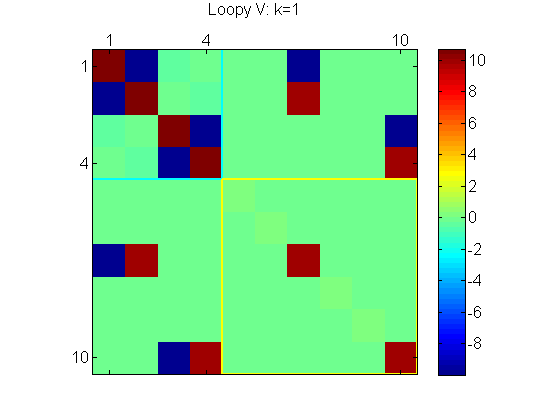
\includegraphics[width=0.45\textwidth]{K1-1.fig}
% \label{subfig:k1-1}
% }
% \subfigure[]{
% 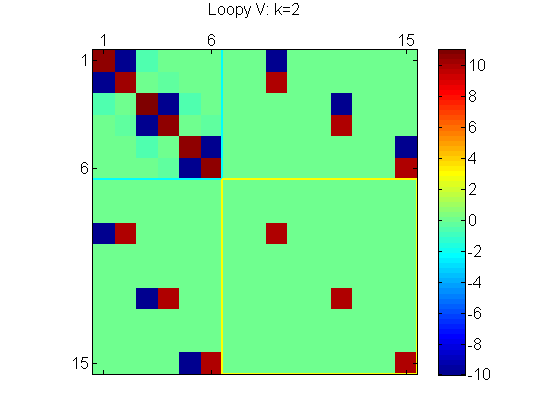
\includegraphics[width=0.45\textwidth]{K2-1}
% \label{subfig:k2-1}
% }
% \subfigure[]{
% 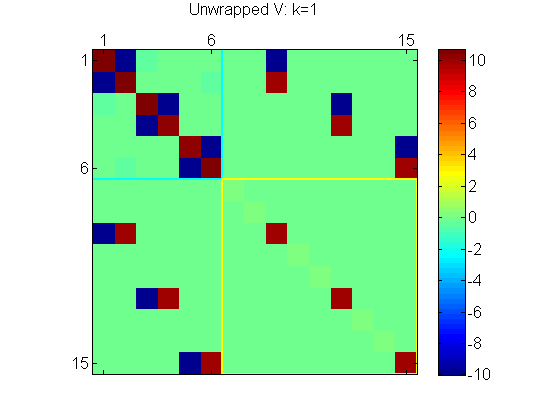
\includegraphics[width=0.45\textwidth]{K1-2}
% \label{subfig:k1-2}
% }
% \subfigure[]{
% 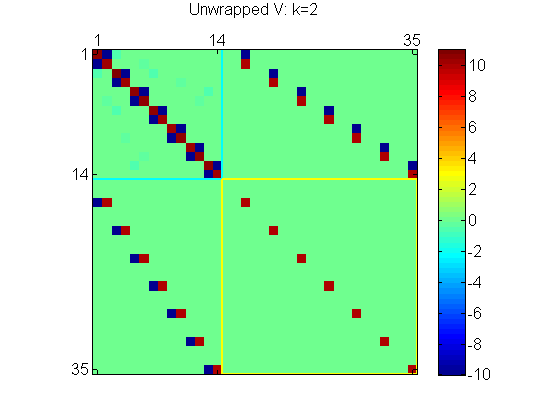
\includegraphics[width=0.45\textwidth]{K2-2}
% \label{subfig:k2-2}
% }
% \subfigure[]{
% 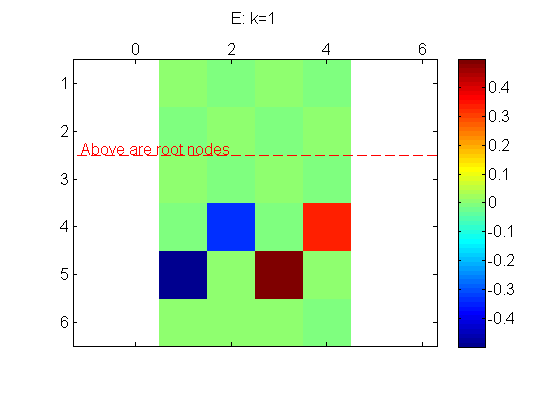
\includegraphics[width=0.45\textwidth]{K1-3}
% \label{subfig:k1-3}
% }
% \subfigure[]{
% 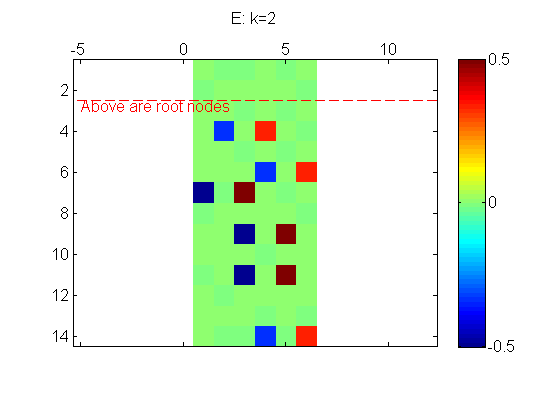
\includegraphics[width=0.45\textwidth]{K2-3-}
% \label{subfig:k2-3}
% }
% \caption{Precision matrices and error matrices for $k=1$ (left column) and $k=2$ (right column).}
% \label{fig:matrices}
% \end{center}
% \end{figure}


% If we rearrange the node sequence in the unwrapped state vector for $k=2$ such that $\tilde{\bf x}=[\tilde{x}_{A,2}^\top, \tilde{x}_{B,2}^\top,\tilde{x}_{A,1}^\top, \tilde{x}_{B,1}^\top,\tilde{x'}_{A,1}^\top, \tilde{x'}_{B,1}^\top,\tilde{x}_{A,0}^\top, \tilde{x}_{B,0}^\top, \tilde{x'}_{A,0}^\top, \tilde{x'}_{B,0}^\top, \tilde{x''}_{A,0}^\top, \tilde{x''}_{B,0}^\top, \tilde{x'''}_{A,0}^\top, \tilde{x'''}_{B,0}^\top]^\top$ (we rearrange the sequence of $y$ accordingly), we can see in Figure~\ref{fig:matrices-re} that the error matrix $\bf E$ is simply adding rows of difference to the $\bf E$ for $k=1$. In this case, the mapping matrix ${\bf O}_{\bf x}=\left[
%              \begin{array}{ccc}
%               \bf 1 & \bf 0 & \bf 0 \\
%               \bf 0 & \bf 1 & \bf 0 \\
%               \bf 0 & \bf 1 & \bf 0 \\
%                 \bf 0 & \bf 0 & \bf 1 \\
%               \bf 0 & \bf 0 & \bf 1 \\
%               \bf 0 & \bf 0 & \bf 1 \\
%               \bf 0 & \bf 0 & \bf 1 \\
%              \end{array}
%           \right]
% $.
% \begin{figure}[H]
% \begin{center}
% \subfigure[]{
% 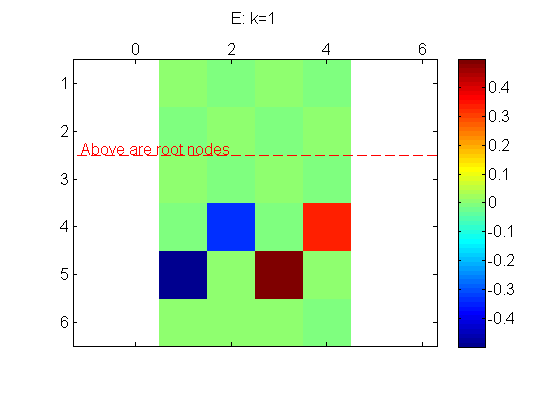
\includegraphics[width=0.45\textwidth]{K1-3}
% \label{subfig:k1-3}
% }
% \subfigure[]{
% 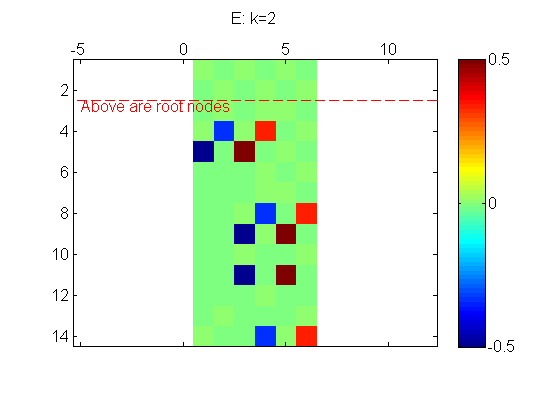
\includegraphics[width=0.45\textwidth]{K2-3}
% \label{subfig:k2-3}
% }
% \caption{Error matrices for $k=1$ (left column) and $k=2$ with rearranged states (right column).}
% \label{fig:matrices-re}
% \end{center}
% \end{figure}
% If you read Yair Weiss paper, there is a difference in unwrapping the original problem. In his paper, the original full network is unwrapped in a way that all non-leaf nodes in the unwrapped structure maintain the same neighboring statistical relationship. We do not have that in our DKF estimation. We assume that all the duplicated nodes for relative measurement updates have no statistical relationship with the future nodes.

% A naive extended Kalman filter (NEKF) does not track the correlation among vehicles; they are always assumed to be independent to one another. This results in a double-counting of information as one vehicle's state may have been used previously. Inconsistent estimate appears where vehicles are overconfident about its own positioning. In this case, less information will be gained from some accurate and important measurements.
% Suboptimal estimation with unknown correlation

% example of information double counting in paper.

% \begin{itemize}

%   \item information flow in partially connected network
% \item Turbo decoder etc for iterative decoding algorithm

% \end{itemize}

\subsection{Multi-Vehicle Localization with Bathymetric Aids}

The multi-vehicle localization consists of vehicles estimating their own positions, and cooperating with an additional relative measurement relating the two vehicles. When bathymetry map is used to assist the localization, the local measurements consist of water depth measurements, and they are fairly accurate. We look at conditions under which correlation can be ignored.

We consider the recursive two-step process where two vehicles (Vehicle $i=1$ and $j=2$) localize themselves (position states ${\bf x}^{(1)}$ and ${\bf x}^{(2)}$) respectively. Similarly we denote previous time step $k$ and current time step $k+1$. At each step, each node makes a local observation (${\bf z}^{(1)}$ or ${\bf z}^{(2)}$) about their respective positions. A range measurement ${\bf r}$ is made between vehicles. The propagation model in Equation~\eqref{eq:mvlpropagation} is simplified as a random walk process
\begin{equation}
\begin{split}
{\bf x}_{k+1}^{(1)}&={\bf x}_k^{(1)}+{\bf \omega}_k^{(1)}\\
{\bf x}_{k+1}^{(2)}&={\bf x}_k^{(2)}+{\bf \omega}_k^{(2)}.\\
\end{split}
\end{equation}
The propagation noises are independent of each other with the same error covariance ${\bf Q}$. The measurements ${\bf z}_k^{(1)}$, ${\bf z}_k^{(2)}$ and $r_k$ in Equation~\eqref{eq:mvlmeasurement} have error covariance ${\bf R}^{(1)}$, ${\bf R}^{(2)}$ and ${\bf R}_r$ respectively. Without loss of generality, we assume ${\bf R}^{(1)}\leq{\bf R}^{(2)}$.
%and at each step we have
%\begin{equation}
 %   \begin{split}
  %      {\bf z}_1&={\bf x}_1+{\bf \nu}_1 \\
%{\bf z}_2&={\bf x}_2+{\bf \nu}_2\\
%r&={\bf x}_1-{\bf x}_2+\upsilon\\
%\end{split}
%\end{equation}
%where the propagation noise $\bf \omega$ and observation noises ${\bf \nu}_1$, ${\bf \nu}_2$ and $\bf\upsilon$ are independent zero-mean Gaussian processes with covariances ${\bf Q}$, ${\bf R}^{(1)}$, ${\bf R}^{(2)}$ and $\bf R$. Without loss of generality, we assume ${\bf R}^{(1)}\leq{\bf R}^{(2)}$. 

Compared with multi-sensor tracking problem, there are two differences. The first difference lies in an additional variable called ranging $r$ at each step. It relates the two position variables. The second difference comes from individual process noise on position of each vehicle. $\omega_1$ and $\omega_2$ are independent noises.% Large propagation noises increase the inter-vehicle independence.

In step $k$, the estimates at Vehicle $i$ and $j$ are ${\bf y}_k^{(1)}$ and ${\bf y}_k^{(2)}$, with the same error covariance ${\bf P}_k$ and correlation coefficient $\rho_k$. Central KF stacks the two state variables and the centralized error covariance is therefore 
%\begin{equation}
 %   \begin{split}
 %       {\bf\bar y}_1&={\bf\bar x}_1+\bar\varepsilon_1 \\
   %     {\bf\bar y}_2&={\bf\bar x}_2+\bar\varepsilon_2.
  %  \end{split}
%\end{equation}
%The estimation error $\bar\varepsilon_1$ and $\bar\varepsilon_2$ are assumed to have covariance ${\bf\bar P}$ and correlation coefficient $\bar\rho$. The central KF stacks the state variables with error covariance in the previous step as 
$\left[
          \begin{array}{cc}
            {\bf P}_k & \rho_k{\bf P}_k \\
            \rho_k{\bf P}_k & {\bf P}_k\\
          \end{array}
        \right]$. Figure~\ref{fig:CKFeg1} and Figure~\ref{fig:CKFeg2} show two examples of centralized processing, with respect to different values of $\rho_k$ and ${\bf R}_r$. The different settings of the two cases have a common extreme situation: when the ranging error is 0, the two estimates are fully correlated (and therefore have the same error covariance) after cooperation. When the ranging error approaches zero, the two estimates are almost fully correlated with similar error covariance after cooperation.
        
         \begin{figure}[htbp]
\begin{center}
\subfigure[Case 1: Correlation coefficient in one-step cooperation.]{
\includegraphics[width=.8\textwidth]{Figures/CKFrhoVSr.pdf}
\label{subfig:CKFrho}
}
\subfigure[Case 1: Error covariances of two vehicles in one-step cooperation.]{
\includegraphics[width=.8\textwidth]{Figures/CKFp.pdf}
\label{subfig:CKFp}
}
\caption{Case 1: ${\bf P}_k=5,{\bf Q}=10,{\bf R}^{(1)}=1,{\bf R}^{(2)}=2$. When ranging error approaches 0, the two estimates are about fully correlated with similar error covariances after cooperation.}
\label{fig:CKFeg1}
\end{center}
\end{figure}

\begin{figure}[htbp]
\centering
\subfigure[Case 2: Correlation coefficient in one-step cooperation.]{
\includegraphics[width=.8\textwidth]{Figures/CKFrhoVSr2.pdf}
\label{subfig:CKFrho2}
}
\subfigure[Case 2: Error covariances of two vehicles in one-step cooperation.]{
\includegraphics[width=.8\textwidth]{Figures/CKFp2.pdf}
\label{subfig:CKFp2}
}
\caption{Case 2:${\bf P}_k=5,{\bf Q}=1,{\bf R}^{(1)}=10,{\bf R}^{(2)}=40$. When ranging error approaches 0, the two estimates are about fully correlated with similar error covariances after cooperation.}
\label{fig:CKFeg2}
\end{figure}

We also analyze the performance of SF, NF and DF (with a weighting factor). A SF at Vehicle 1 has
\begin{equation}
\begin{split}
    {\bf y}^{(1)}_{k+1}&={\bf y}_k^{(k)}+({\bf P}_k+{\bf Q}^{(1)})({\bf P}_k+{\bf Q}^{(1)}+{\bf R}^{(1)})^{-1}({\bf z}^{(1)}_{k+1}-{\bf y}^{(1)}_{k+1}) \\
    {\bf P}^{(1)}_{k+1}&=({{\bf P}_k}^{-1}+{{\bf R}^{(1)}}^{-1})^{-1}. \\
\end{split}
\end{equation}
This is standard KF and Vehicle 2 obtains its estimation in the same way. NF fuses the estimated position from Vehicle 2 about Vehicle 1 such that ${\bf y}^{(1)}_{\text{NF}}=\lambda_\text{NF}{\bf y}^{(1)}_{k+1}+(1-\lambda_\text{NF})({\bf y}^{(2)}_{k+1}+{r}_{k+1})$, where the weight $\lambda_\text{NF}=({\bf P}^{(2)}_{k+1}+{\bf R}_r)({\bf P}^{(1)}_{k+1}+{\bf P}^{(2)}_{k+1}+{\bf R}_r)^{-1}$.

DF fuses the estimated position from Vehicle 2 using a weight $\lambda_1$ such that ${\bf y}^{(1)}_{\text{DF}}=(1-\lambda_1){\bf y}^{(1)}_{k+1}+\lambda_1({\bf y}^{(2)}_{k+1}+r_{k+1})$. At Vehicle 2, the DF fuses the estimated position from Vehicle 1 using a weight $\lambda_2$ such that ${\bf y}^{(2)}_{\text{DF}}=(1-\lambda_2){\bf y}^{(2)}_{k+1}+\lambda_2({\bf y}^{(1)}_{k+1}-{r}_{k+1})$. The error covariances can be calculated accordingly. The optimal weights can be obtained such that
\begin{equation}
\begin{split}
    \lambda_1^*&=\arg\min\mathbb{E}[({\bf y}^{(1)}_{\text{DF}}-{\bf x}^{(1)}_{k+1})^2]\\
    \lambda_2^*&=\arg\min\mathbb{E}[({\bf y}^{(2)}_{\text{DF}}-{\bf x}^{(2)}_{k+1})^2].\\
\end{split}
\label{eq:mvlDF}
\end{equation}
When ranging error ${\bf R}_r=0$, we have $\lambda_1^*+\lambda_2^*=1$ and the two estimates are fully correlated after cooperation. When the ranging error ${\bf R}_r$ is very small, $\lambda_1^*+\lambda_2^*$ also approaches 1. In underwater communications, we do have the ability to achieve very small ranging error, compared with positioning error. For simplicity, we set ${\bf R}_r=0$ and therefore the correlation coefficient goes to 1.

\subsubsection{One-Step Performance}

We calculate the one-step \textit{dangerous} region, similar to the situation in Equation~\eqref{eq:nffail}, that is
\begin{equation}
 \det\mathbb{E}[({\bf y}^{(1)}_{\text{NF}}-{\bf x}_{k+1})({\bf y}^{(f)}_{\text{NF}}-{\bf x}_{k+1})^\top]>\det{\bf P}_{k+1}^{(1)}.  
 \label{eq:mvlnffail}
\end{equation}

Firstly, we consider the extreme cases. When ${\bf Q}\rightarrow 0$, the inequality is the same as Equation~\eqref{eq:danger} except that the normalized ${\bf\bar R}^{(i)}=\frac{{\bf R}^{(i)}}{{\bf P}_k}$. It has the same region in the two-sensor tracking problem. This is easy to understand as the zero propagation noise makes the two states fully correlated. In such a case, we can see that the DF has the optimal weight $\lambda^*_\text{DF}=\frac{{\bf R}^{(1)}}{{\bf R}^{(1)}+{\bf R}^{(2)}}$. The same result can be derived by minimizing the error covariance in Equation~\eqref{eq:mvlDF}.

When ${\bf Q}\gg{\bf P}_k$ and ${\bf R}^{(i)}\ll{\bf Q}$, NF approaches the performance of CF, because the assumption of independence is almost valid. We can ignore the correlation.

When the propagation noise is neither too small nor too large, we derive the \textit{dangerous} region shown in Figure~\ref{fig:mvlOneStepRegion} when Equation~\eqref{eq:mvlnffail} is met. This region tells us when the local propagation error is small, the states are more correlated. Vehicle 2 maintains most of the correlated information when ${\bf R}^{(2)}>{\bf R}^{(1)}$. In such a case, if the correlation in the estimate from Vehicle 2 is ignored, the fused estimate is worse than the estimate from SF.

\begin{figure}[htbp]
  \centering
    \includegraphics[width=.8\textwidth]{Figures/mvlOneStepRegion.pdf}
      \caption{One-step Performance: The \textit{dangerous} region of implementing NF in multi-vehicle localization. (${\bf\bar R}^{(2)}>{\bf\bar R}^{(1)}$)}
      \label{fig:mvlOneStepRegion}
\end{figure}


\subsubsection{Asymptotic Performance}

Figure~\ref{fig:sscases} shows the estimation performance in stable state. The cases are located in Figure~\ref{fig:mvlssRegion} using their parameter values. The normalized ${\bf\bar R}^{(i)}={\bf R}^{(i)}/{\bf Q}$. In the three cases, cooperative localization with bathymetric aids is most similar to Case (b) and Case (c). The relative distance measured by acoustic signals has small error (${\bf R}_r$ is in the sub-meters range); the local measurement, i.e., the water depth has much smaller errors compared with the propagation errors accumulated between cooperation. Even if any one of the cooperative vehicles has little or none of the bathymetry aids (large measurement error like Case (c)), it is still safe to ignore the correlation.

\begin{figure}[htbp]
\centering
\subfigure[Actual error covariance eventually grows larger than SF.]{
\includegraphics[width=.6\textwidth]{Figures/sscasea.png}
\label{subfig:sscasea}
}
\subfigure[It is safe to ignore correlation and the performance is close to CF.]{
\includegraphics[width=.6\textwidth]{Figures/sscaseb.png}
\label{subfig:sscaseb}
}
\subfigure[Actual error covariance is smaller than SF but the estimation is overconfident.]{
\includegraphics[width=.6\textwidth]{Figures/sscasec.png}
\label{subfig:sscasec}
}
\caption{\textit{Na\"ive} filter in stable state: One can ignore the correlation in Case (b) and Case (c) but NF becomes detrimental in Case (a).}
\label{fig:sscases}
\end{figure}

\begin{figure}[htbp]
  \centering
    \includegraphics[width=.8\textwidth]{Figures/mvlssregion.pdf}
      \caption{Asymptotic Performance: The \textit{dangerous} region of implementing NF in multi-vehicle localization. The three cases in Figure~\ref{fig:sscases}are located in the regions.}
      \label{fig:mvlssRegion}
\end{figure}

\section{Summary}

We demonstrated why there is information loss in distributed localization, and how the information is double counted if one ignores the correlation.

For a cooperation method, when the actual localization is worse than single-vehicle localization, we call it \textit{dangerous} as this cooperation makes the estimation worse. When the actual localization is better than single-vehicle localization, we perceive it safe as this cooperation helps. For both types of cooperative localization - multi-sensor tracking problem and multi-vehicle localization problem, we quantified the safe and \textit{dangerous} regions when ignoring correlation during fusion. This can be used as a guideline to justify the \textit{na\"ive} assumption. The \textit{na\"ive} assumption is justified safe to use in cooperative localization with bathymetric aids in the next chapter.